\section*{Лекция 7 (31.03.2022)}

5. (дифференциал обратного отображения)


$X, Y$ --- нормированные пространсвтва

$U \subset X, V \subset Y$ --- открытые

$f: U \to V$ --- биекция

$x_0 \in U, y_0 = f(x_0) \in V$

$f $ --- непр в $(\cdot) x_0$, $f^{-1}$ непр. в $(\cdot) y_0$

$f$ --- дифференцируема в $(\cdot)x_0$, $\exists (df(x_0))^{-1} \in L(Y, X)$

$\hence f^{-1}$ дифф. в $(\cdot) y_0$ и $df^{-1}(y_0) = (df(x_0))^{-1}$


\begin{proof}
    $f(x_0 + h) - f(x_0) = k$, $f(x_0 + h) = y_0 + k$, $h = f^{-1}(y_0 + k) - \underbrace{f^{-1}(y_0)}_{=x_0}$

    $h \to 0 \Longleftrightarrow k \to 0$

    $k = f(x_0 + h) - f(x_0) = df(x_0)h + o(h)$ | применяем $(df(x_0))^{-1}$

    $(df(x_0))^{-1} k = \underbrace{f^{-1}(y_0 + k) - f^{-1}(y_0)}_{=h} + (df(x_0))^{-1}(o(h)) \Longleftrightarrow f^{-1}(y_0 + k) - f^{-1}(y_0) = (df(x_0)) ^ {-1} k + \underbrace{(df(x_0))^{-1}(o(h))}_{?= o(k)}$

    $\norm{df(x_0)^{-1}(o(h))} \leqslant C \norm{o(h)} = o(h)$

    $\hence o(h) \underset{?}{=} o(k) \Longleftrightarrow \begin{cases}
        \norm{h} \leqslant C \norm{k} \\
        \norm{k} \leqslant C\norm{h}
    \end{cases}$

    $k = f(x_0 + h) - f(x_0) = df(x_0)h + o(h) \hence \norm{k} \leqslant \norm{df(x_0)} \cdot \norm{h} + \norm{o(h)} \leqslant C \norm{h}$

    $(df(x_0))^{-1} k = \underbrace{f^{-1}(y_0 + k) - f^{-1}(y_0)}_{=h} + (df(x_0))^{-1}(o(h)) \Longleftrightarrow h = (df(x_0))^{-1}k + (df(x_0))^{-1}(o(h))$

    $\norm{h} \leqslant c \norm{k} + \frac{1}{2}\norm{h}$ при дост.мал.h $\hence \norm{h} \leqslant C \norm{k}$
\end{proof}
\newpage

\begin{examples}
\begin{enumerate}
    \item (постоянное отображение) $f: X \to Y$, $f(x) \equiv y_0 \hence \forall x df(x) = 0$
    \item (линейное) $f \in L(X, Y), df(x) = f$, $(df(x)h = f(h))$
    \item (композиция c лин.) $f : X \to Y, f$ дифф. в $(\cdot) x_0$, $A \in L(Y, Z)$ 
        $ \hence d(A \circ f)(x_0) = Adf(x_0)$
    \item $f : X \to Y_1 \times Y_2 \times ... \times Y_n$, $f(x) = (f_1(x), f_2(x), ..., f_n(x))$, $f_j$ --- координатные отображения $f$
    
    $f$ --- дифференцируема в $(\cdot) x_0 \Longleftrightarrow $ все $f_j $ дифференцируемы в $(\cdot) x_0$

    $df(x_0) = (df_1(x_0), ..., df_n(x_0))$, $\left( df(x_0)h = (df_1(x_0)h, ..., df_n(x_0)h) \right)$

    $f(x_0 + h) - f(x_0) = (f_1(x_0 + h) - f_1(x_0), ... , f_n(x_0 + h) - f_n(x_0))$

    $\ora = df(x_0)h + o(h) = (A_1h + o(h), ... , A_nh + o(h)) \hence f_j$ дифф. $A_j = df_j(x_0)$

    $\ola f(x_0 + h) - f(x_0) - (df_1(x_0)h + o(h), ... ) = \underbrace{(df_1(x_0) h, ... , df_n(x_0) h)}_{Ah} + o(h), A \in L(X, Y_1 \times Y_2 \times ... \times Y_n)$


    \item $\underbrace{X_1 \times X_2 \times ... \times X_n }_{(x_1, ... , x_n)}\to \underbrace{X_j}_{x_j}$
    
    $x_j : (x_1, ..., x_n) \to x_j$

    $dx_j(x) : (h_1, ..., h_n) \to h_j$
            
    \item $A : X_1 \times ... \times X_n \to Y$ --- непр. полилинейное отображение
    
    $h = (h_1, ..., h_n)$

    $dA(x)h = A(x_1, h_2) + A(h_1, x_2) \hence dA = A(dx_1, ..., x_n) + A(x_1, dx_2, ..., x_n) + ... + A(x_1, ..., x_{n- 1}, dx_n)$

    $A(x + h) - A(x) = A(x_1 + h_1, x_2 + h_2) - A(x_1, x_2) = \underbrace{A(x_1, h_2) + A(h_1, x_2)}_{\text{лин. по } h} + \underbrace{A(h_1, h_2)}_{=o(h)}$

    \underline{Частные случаи} 

    \begin{enumerate}
        \item $f : \R \times \R ... \R \to \R$
        
        $(x_1, ..., x_n) \to x_1 \cdot \ldots \cdot x_n$

        $d(x_1 \cdot...\cdot x_n) = x_2 \cdot ... \cdot x_n dx_1 + ... + x_1 \cdot x_2 ... x_{n - 1} dx_n$

        \item $f, g : X \to \R (\mathbb{C})$, дифференцируемые в $(\cdot)x_0$, $dfg(x_0) = f(x_0)dg(x_0) + g(x_0) df(x_0)$, $d(fg) = fdg + gdf$
        
        План: $x \underset{F}{\to} (f(x), g(x)) \underset{A}{\to} f(x) g(x)$

        $dF(x_0) = (df(x_0), dg(x_0)) \hence dF(x_0)h = (df(x_0)h, dg(x_0)h)$

        $dA(f(x_0), g(x_0))h = A(f(x_0), h_2) + A(h_1, g(x_0)) = f(x_0)h_2 + h_1g(x_0)$

        $G = A \circ F$

        $dG(x_0)h = f(x_0)dg(x_0)h + g(x_0)df(x_0)h$

        \item $f, g : X \to R^n, d \langle f, g \rangle = \langle df, g \rangle + \langle f, dg \rangle$
    
        $X \to (f, g) \to \langle f, g \rangle$

        \item $det$ $\underbrace{\R ^ n \times ... \times \R^n}_{n} \to \R$ (его можно по аналогии продифференцировать)
        
        \item $f, g : X \to R^3$, $d[f, g] = [df, g] + [f, dg], 
        [u, v] - $ векторное произведение
        
    \end{enumerate}
\end{enumerate}

\underline{Задача} 

$Y \subset L(X, X)$, $U \in Y \Longleftrightarrow \exists u^{-1} \in L(X, X)$

\begin{enumerate}
    \item Y --- открыто
    \item $f : U \to U^{-1} \hence f$ дифференцируема $df = ?$
\end{enumerate}
    

\end{examples}

\newpage

\subsection{Частные дифференциалы (производные)}

\begin{definition}
    $a \in U \text{ --- открытое} \subset X_1 \times X_2 \times ... \times X_m$,
     $f : U \to Y$, $X_1, ..., X_m, Y$
      ---  линейные нормированные пространсвтва над одним полем скаляров.

    $a = (a_1, ..., a_m)$

    $\phi_j(x_j) = f(a_1, ..., x_j, ..., a_m)$

    $\phi_j : X_j \to Y$



\tikzset{every picture/.style={line width=0.75pt}} %set default line width to 0.75pt        

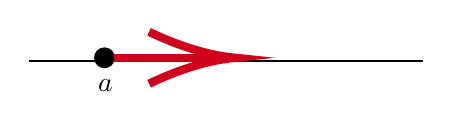
\begin{tikzpicture}[x=0.75pt,y=0.75pt,yscale=-1,xscale=1]
%uncomment if require: \path (0,300); %set diagram left start at 0, and has height of 300

%Straight Lines [id:da4887794321958592] 
\draw    (100,115) -- (290,115) ;
%Shape: Circle [id:dp9534128776661086] 
\draw  [fill={rgb, 255:red, 0; green, 0; blue, 0 }  ,fill opacity=1 ] (132,113.5) .. controls (132,111.01) and (134.01,109) .. (136.5,109) .. controls (138.99,109) and (141,111.01) .. (141,113.5) .. controls (141,115.99) and (138.99,118) .. (136.5,118) .. controls (134.01,118) and (132,115.99) .. (132,113.5) -- cycle ;
%Straight Lines [id:da3314315375931488] 
\draw [color={rgb, 255:red, 208; green, 2; blue, 27 }  ,draw opacity=1 ][line width=3]    (141,113.5) -- (194.5,113.5) ;
\draw [shift={(199.5,113.5)}, rotate = 180] [color={rgb, 255:red, 208; green, 2; blue, 27 }  ,draw opacity=1 ][line width=3]    (41.53,-12.5) .. controls (26.41,-5.31) and (12.57,-1.14) .. (0,0) .. controls (12.57,1.14) and (26.41,5.31) .. (41.53,12.5)   ;

% Text Node
\draw (132,122.4) node [anchor=north west][inner sep=0.75pt]    {$a$};


\end{tikzpicture}

    Если $\phi_j$ дифф в $(\cdot) a_j$, то $d\phi_j(a_j)$ --- частный дифференциал $f$ по $x_j$ в точке a

\underline{Обозначения} $\partial_{x_j} f(a) = D_{x_j} f(a) = \frac{\partial f}{\partial x_j}(a) = \partial_jf(a) = f_{x_j}'(a) $

$d_{x_j}f(a) \in L(x_j, Y)$
\end{definition}

\begin{statement}
    $f$ дифф в $(\cdot) a \hence \exists$ все частные дифференциалы в $(\cdot) a$

    $df(a)h = \partial_{x_1}f(a)h_1 + ... + \partial_{x_m}f(a)h_m, h = (h_1, ..., h_m)$
\end{statement}

\begin{proof}
    $f(a + h) - f(a) = df(a)h + o(h)$ 

    $h = (h_1, 0, 0, ..., 0)$

    $\underbrace{f(a + h) - f(a)}_{ = df(a)h + o(h)} = \phi_1(a_1 + h_1) - \phi_1(a_1) \hence \phi_1$ дифф. в $(\cdot) a_1$ и 
    $\underbrace{d_{\phi_1}(a_1)h_1}_{\partial_{x_1} f(a)h_1} = df(a)(h_1, 0, 0, ...)$  

    Далее просто представляем $h = (h_1, 0, ..., 0) + (0, h_2, 0, ..., 0) + ...$ и получаем искомую сумму.
\end{proof}

\underline{Очень важный частный случай}

$f : \R ^ m \to \R^n$

\begin{enumerate}
    % \item $f(x) = (f_1(x), ..., f_n(x)) $ дифф. $f$ в $(\cdot) a \Longleftrightarrow $ дифф. всех f_j в $(\cdot) a$
    
    % $df(a) = (df_1(a), ..., df_n(a))$

    \item $f : \R ^ m \to \R$ --- функция
    
    f --- дифф. в $(\cdot)a \hence \exists $ частные производные $\frac{\partial f}{\partial {x_j}}(a) = \partial _{x_j}f(a)$

    $df(a)h = \frac{\partial f}{\partial x_1}(a)h_1 + ... + \frac{\partial f}{\partial x_m}(a)h_m = \left( \frac{\partial f}{\partial x_1}(a), ... , \frac{\partial f}{\partial x_m}(a)\right) \begin{pmatrix}
        h_1\\
        ...\\
        h_m
    \end{pmatrix}$

    \begin{definition}
        $ \nabla f(a) = grad f(a) = \begin{pmatrix}
            \frac{\partial f}{\partial x_1}(a)\\
            ...\\
            \frac{\partial f}{\partial x_m}(a)\\
        \end{pmatrix}$

        $df(a)h = \langle \Delta f(a), h \rangle$
    \end{definition}
\end{enumerate}


\begin{remark}
    $df(a)h = \partial_{x_1}f(a)h_1 + ... + \partial_{x_m}f(a)h_m, h = (h_1, ..., h_m)$ 
    
    $\Longleftrightarrow df(a) = \underbrace{\partial_{x_1}f(a)}_{\in L(X_1, Y)} \underbrace{dx_1}_{\in L(X_1 \times ... \times X_m, X_1)} + ... \partial_{x_m}f(a)dx_m$
    
    $f : \R^ m \to R$, $df(a) \in L(\R ^ m, \R) = \frac{\partial f}{\partial x_1}(a) \underbrace{dx_1}_{\in L(\R^m, \R)} + ... + \frac{\partial f}{\partial x_m}(a) dx_m$
\end{remark}

2. (возвращаемся к 1)

$f : \R ^ m \to \R^n$

$f(x) = (f_1(x), ..., f_n(x))$

$f$ дифференцируема в $(\cdot) a \hence f_j$ дифф. в $(\cdot) a$


$f_j : \R^ m \to \R$

$df(a)h = \begin{pmatrix}
    df_1(a)h\\
    ...\\
    df_n(a)h
\end{pmatrix} = \begin{pmatrix}
    \sum_{j=1}^m \frac{\partial f_1}{\partial x_j}(a) h_j\\
    ...\\
    ... 
\end{pmatrix} = \begin{pmatrix}
    \frac{\partial f_1}{\partial x_1}(a) ... \frac{\partial f_1}{\partial x_m}(a) \\
    \dots \\
    \frac{\partial f_n}{\partial x_1}(a) ... \frac{\partial f_n}{\partial x_m}(a) 
\end{pmatrix} \begin{pmatrix}
    h_1\\
    ...\\
    h_m
\end{pmatrix}$ --- Матрица Якоби $f$ в $(\cdot) a$. \\ \\ Ее определитель --- якобиан


3. $\R^m \underset{f}{\to} \R^n \underset{g}{\to}  \R ^ k$

$b = f(a)$

f дифф в $(\cdot) a$
g дифф в $(\cdot) f(a)$

$\underbrace{\underbrace{\R ^ m}_{x} \underset{df(a)}{\to} \underbrace{\R ^ n}_{y} \underset{dg(b)}{\to} \R ^ k}_{\underset{d(g\circ f)(a)}{\to}}$

$1 \leqslant i \leqslant n$,
$1 \leqslant j \leqslant m$,
$1 \leqslant l \leqslant k$

$\underbrace{\begin{pmatrix}
    \frac{\partial g_l}{\partial y_i}(f(a))
\end{pmatrix}}_{dg(f(a))} \underbrace{\begin{pmatrix}
    \frac{\partial f_i}{\partial x_j}(a)
\end{pmatrix}}_{df(a)} = \underbrace{\begin{pmatrix}
    \frac{\partial (g_l \circ f)}{\partial x_j}(a)
\end{pmatrix}}_{d(g \circ f)(a)}$ --- правило цепочки

$\frac{\partial (g_l \circ f)}{\partial x_j}(a) = \sum_{i = 1}^{n} \frac{\partial g_l}{\partial y_i}(f(a)) \frac{\partial f_i}{\partial x_j}(a)$


$k = 1$

$\frac{\partial (g \circ f)}{\partial x_j}(a) = \sum_{i = 1} ^ n \frac{\partial g}{\partial y_i}(f(a)) \frac{\partial f_i}{\partial x_j}(a)$ (часто бывает $x, y$ просто разные коорд. в $R ^ m$)
